\documentclass{beamer}
\usepackage{multimedia}
\usepackage{hyperref}

% Theme choice
\usetheme{Madrid}

\definecolor{SpaceNavy}{RGB}{11, 19, 43}       % Primary dark background
\definecolor{CosmicIndigo}{RGB}{28, 37, 65}    % Secondary dark tone
\definecolor{NebulaBlue}{RGB}{0, 150, 214}     % Vibrant accent blue
\definecolor{StarGold}{RGB}{255, 183, 3}       % Warm highlight color
\definecolor{DeepSpaceBlack}{RGB}{10, 10, 18}  % Deep structure background

% Set theme elements
\setbeamercolor{structure}{fg=NebulaBlue}
\setbeamercolor{palette primary}{bg=SpaceNavy, fg=white}
\setbeamercolor{palette secondary}{bg=CosmicIndigo, fg=white}
\setbeamercolor{palette tertiary}{bg=DeepSpaceBlack, fg=white}
\setbeamercolor{titlelike}{parent=palette primary, fg=white}
\setbeamercolor{frametitle}{bg=SpaceNavy, fg=white}
\setbeamercolor{item}{fg=NebulaBlue}
\setbeamercolor{subitem}{fg=StarGold}
\setbeamercolor{block title}{bg=CosmicIndigo, fg=white}
\setbeamercolor{block body}{bg=SpaceNavy!10, fg=black}


% makes dark mode
%\setbeamercolor{normal text}{fg=white, bg=DeepSpaceBlack}
%\usebeamercolor[fg]{normal text}


% Title Page Information
\title[H$\gamma$ and $OIII$ in LRDs]{The Relationship Between the [OIII]$\lambda$4363/H$\gamma$ ratio in Little Red Dots
}
\subtitle{Astrophysics}
\author{Kate Bopp} 
\date{July 2026}

\begin{document}

% --- Slide 1: Title Page ---
\begin{frame}
    \titlepage
\end{frame}

% --- Slide 3: Introduction ---
\begin{frame}
    \frametitle{Introduction}
        \centering
        \Large{The question:} 

        \huge{What are Little Red Dots?}
\end{frame}

% --- Slide 3: Spectroscopy ---
\begin{frame}
    \frametitle{Spectroscopy}
        \begin{center} 
        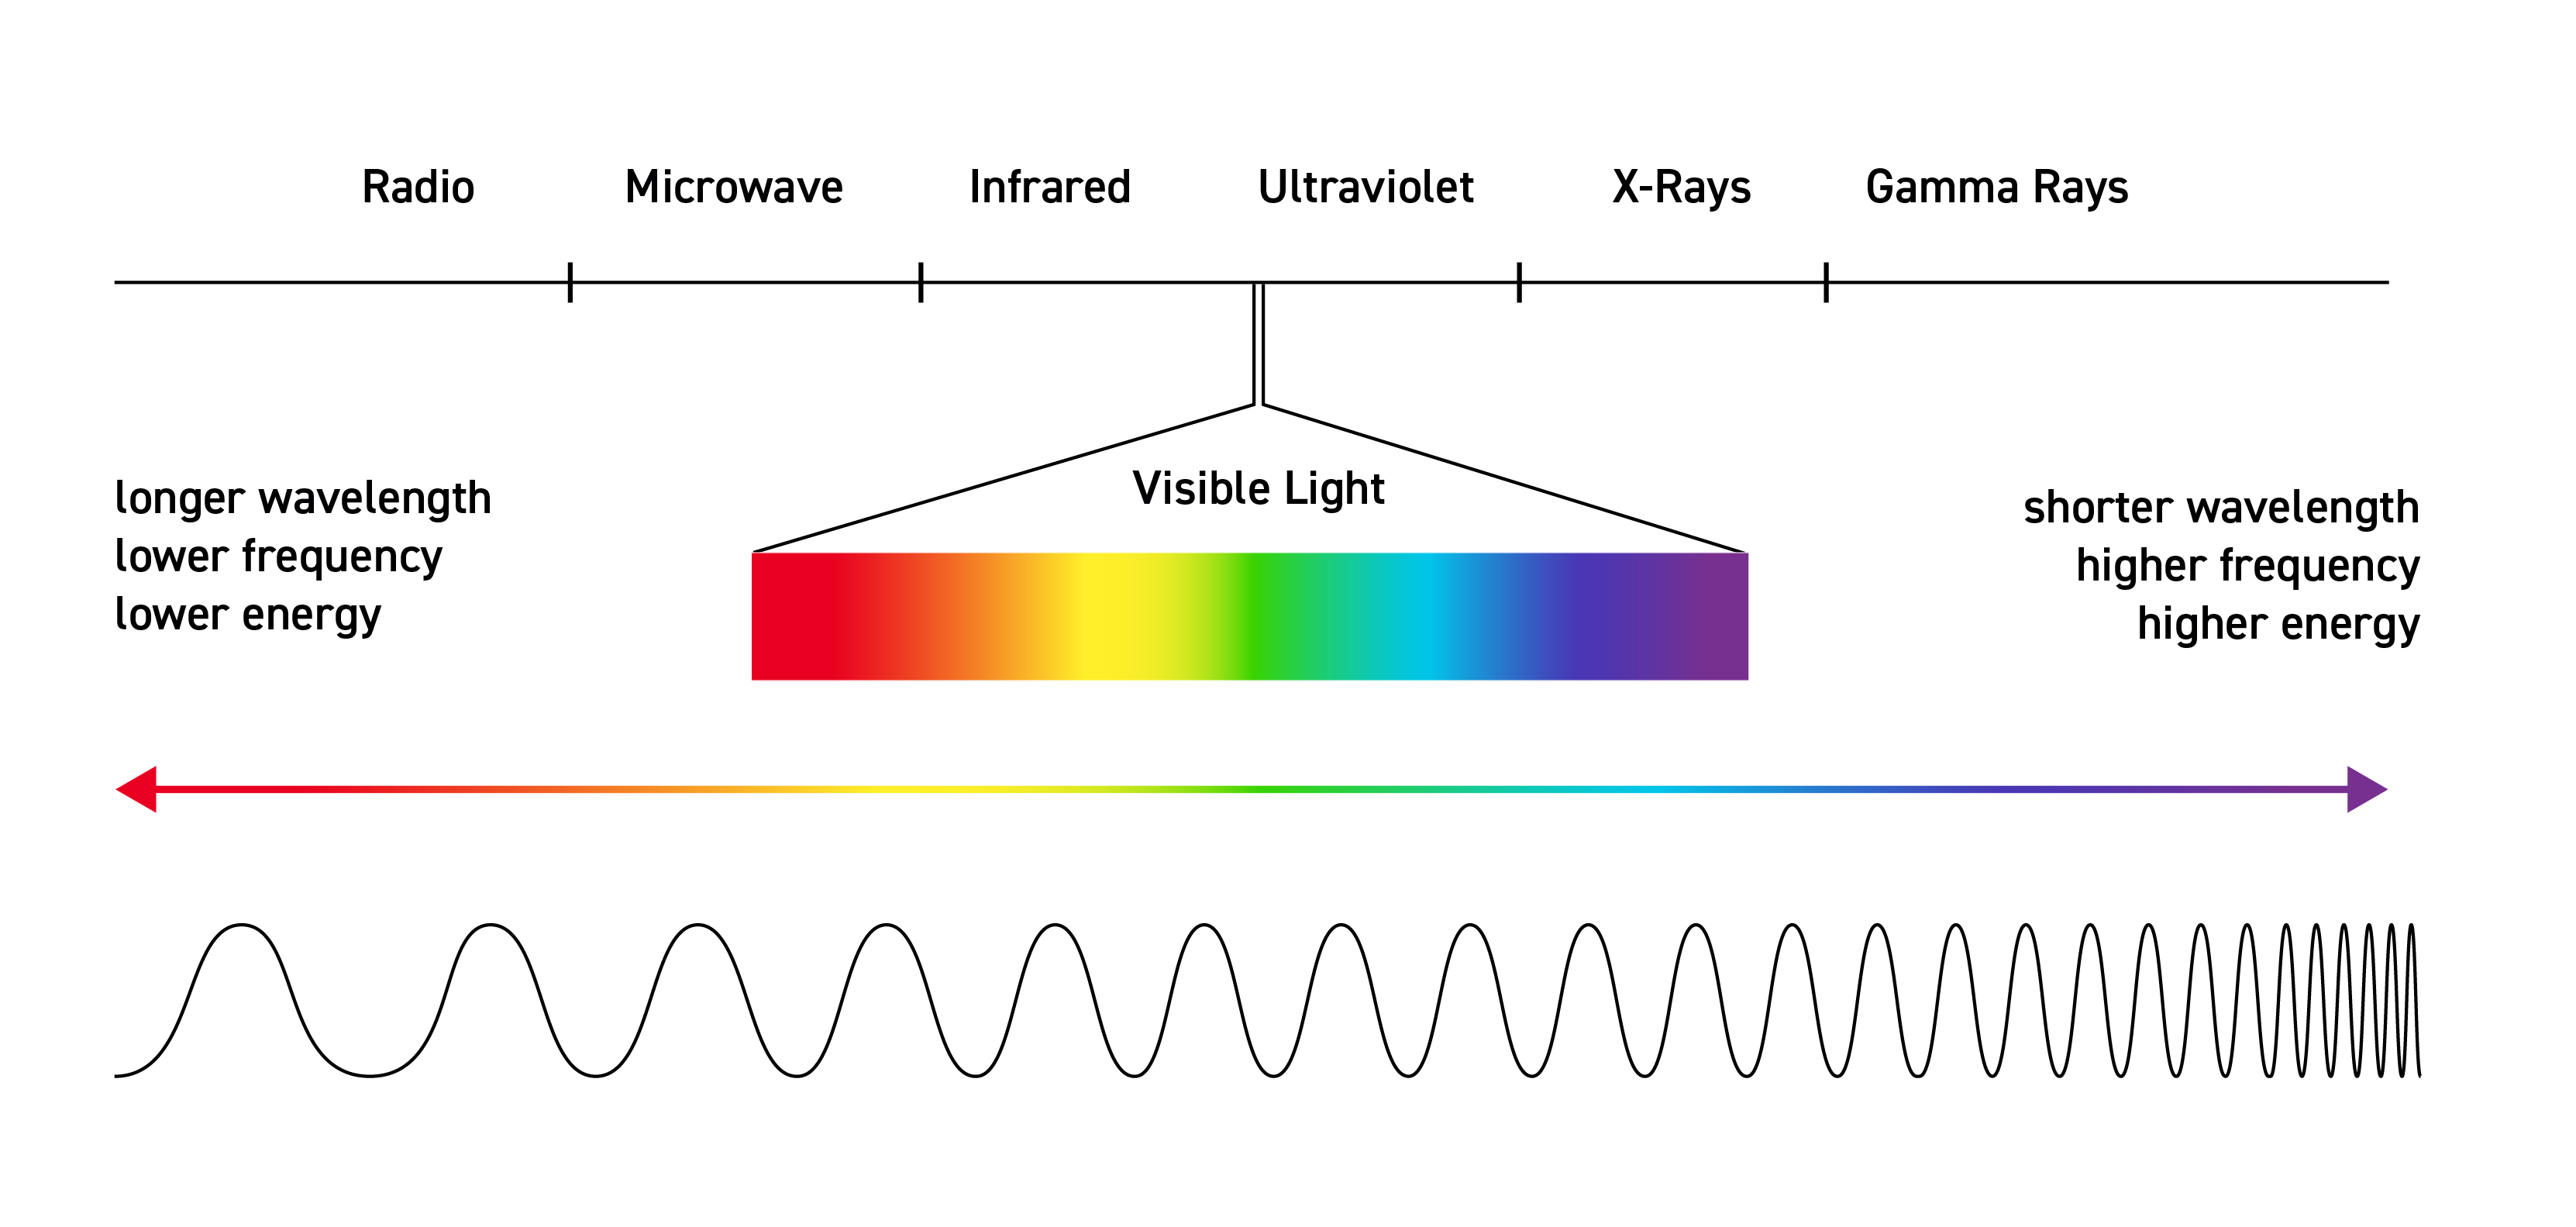
\includegraphics[width=0.7\textwidth]{spectroscopy.png}
        \vspace{0.2cm} % Adds a tiny bit of vertical space so it isn't squished
        \scriptsize \textit{Source: NIST} % Makes the text small and italicized
    \end{center}
    \begin{itemize}
        \item Breaks galaxy light down into individual component wavelengths ($\lambda$) to reveal physical properties.
        \item Smooth continuum vs sharp emission lines
        \vspace{0.3cm}
    \end{itemize}
\end{frame}

% --- Slide 4: The JWST / NIRSpec Observatory ---
\begin{frame}
    \frametitle{The JWST / NIRSpec Observatory}

    % start image
    \begin{center} 
        \includegraphics[width=0.6\textwidth]{jwst.png}
        \vspace{0.2cm} % Adds a tiny bit of vertical space so it isn't squished
        \scriptsize \textit{Source: University of Utah} % Makes the text small and italicized
    \end{center}
    
    \begin{itemize}
        \item JWST: 6.5-meter primary mirror equipped with gold-coated beryllium segments to optimize near-infrared reflection
        \item NIRSpec
    \end{itemize}
    
    \vspace{0.2cm}

\end{frame}

% --- Slide 6: Emission-Line Diagnostic Boundaries ---
\begin{frame}
    \frametitle{Emission-Line Diagnostic Boundaries}
    
    % start image
    \begin{center} 
        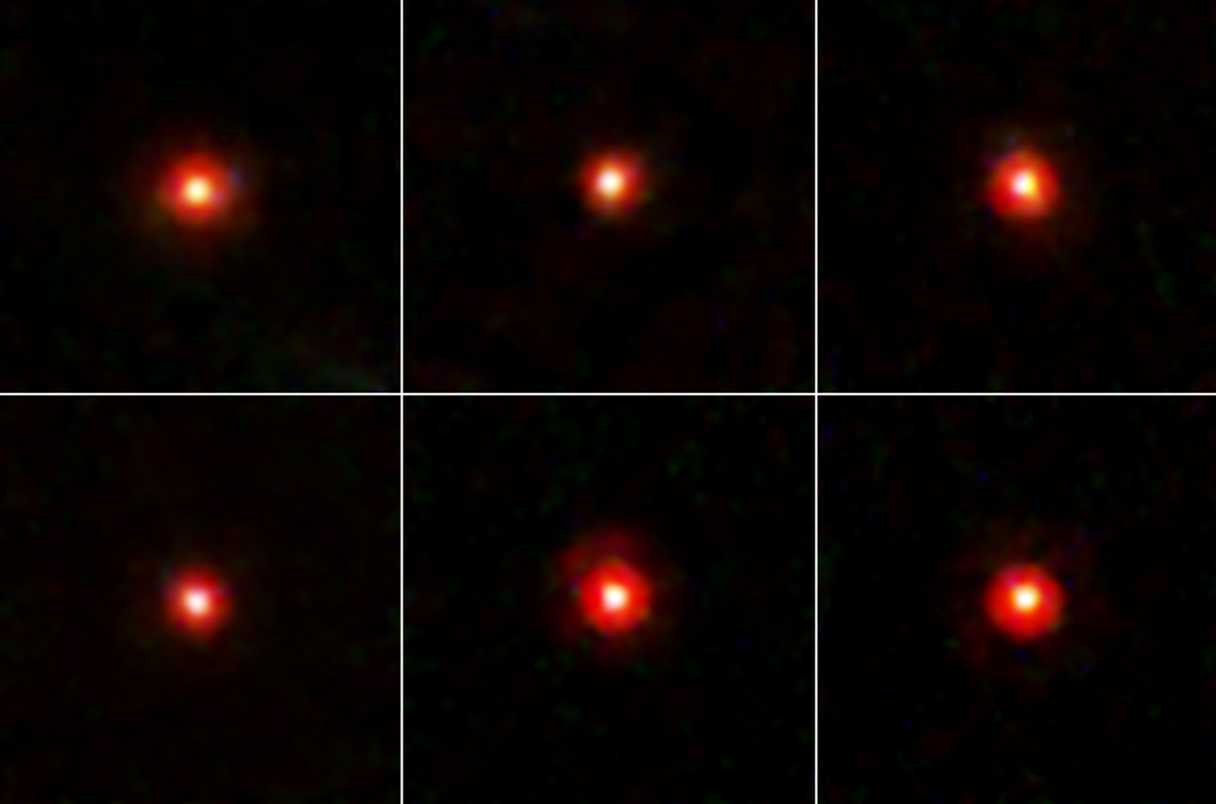
\includegraphics[width=0.5\textwidth]{emission.png}
        \vspace{0.2cm} % Adds a tiny bit of vertical space so it isn't squished
        \scriptsize \textit{Source: NASA;ESA;CSA;STScI;Dale Kocevski/Colby College} % Makes the text small and italicized
    \end{center}
    
    \begin{itemize}
        \item Star-Forming (SF): Lower excitation ($\log_{10} < -0.44$); gas heated by young, massive starbursts
        \item Broad-Line AGN (BLAGN): High excitation ($\log_{10} > -0.26$); hard radiation field powered by accreting supermassive black holes.
        \item Composite: Intermediate excitation ($-0.44 \le \log_{10} \le -0.26$) overlapping star formation and central black hole activity
    \end{itemize}
    
    \vspace{0.2cm}
    
    
\end{frame}

    
% --- Slide 7: Redshift ---
\begin{frame}
    \frametitle{Redshift}
    
    \begin{columns}
            % --- Right Column (Images) ---
        \begin{column}{0.5\textwidth}
            \begin{center}
                % First Image
                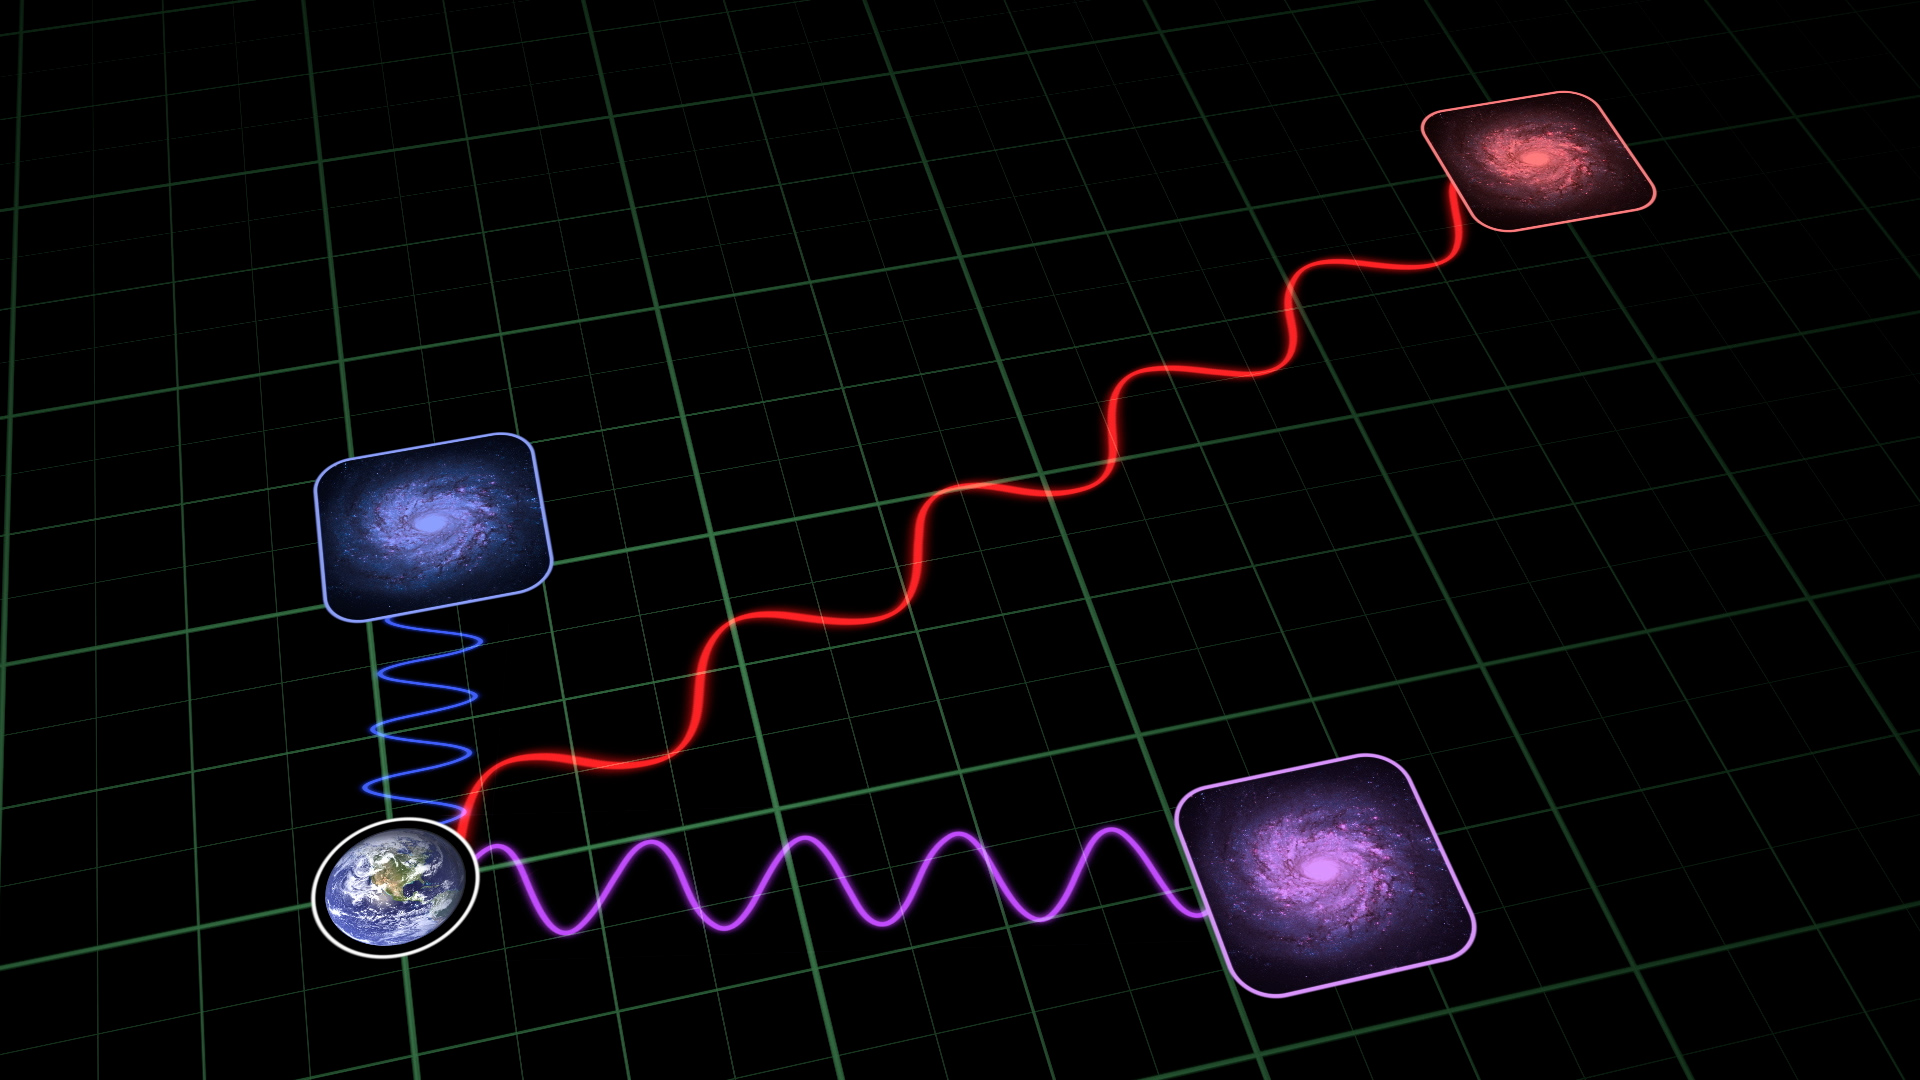
\includegraphics[width=0.8\textwidth]{redshift_3lines.png} \\
                
                \vspace{0.3cm} % Adds a little space between the two images
                
                % Second Image
                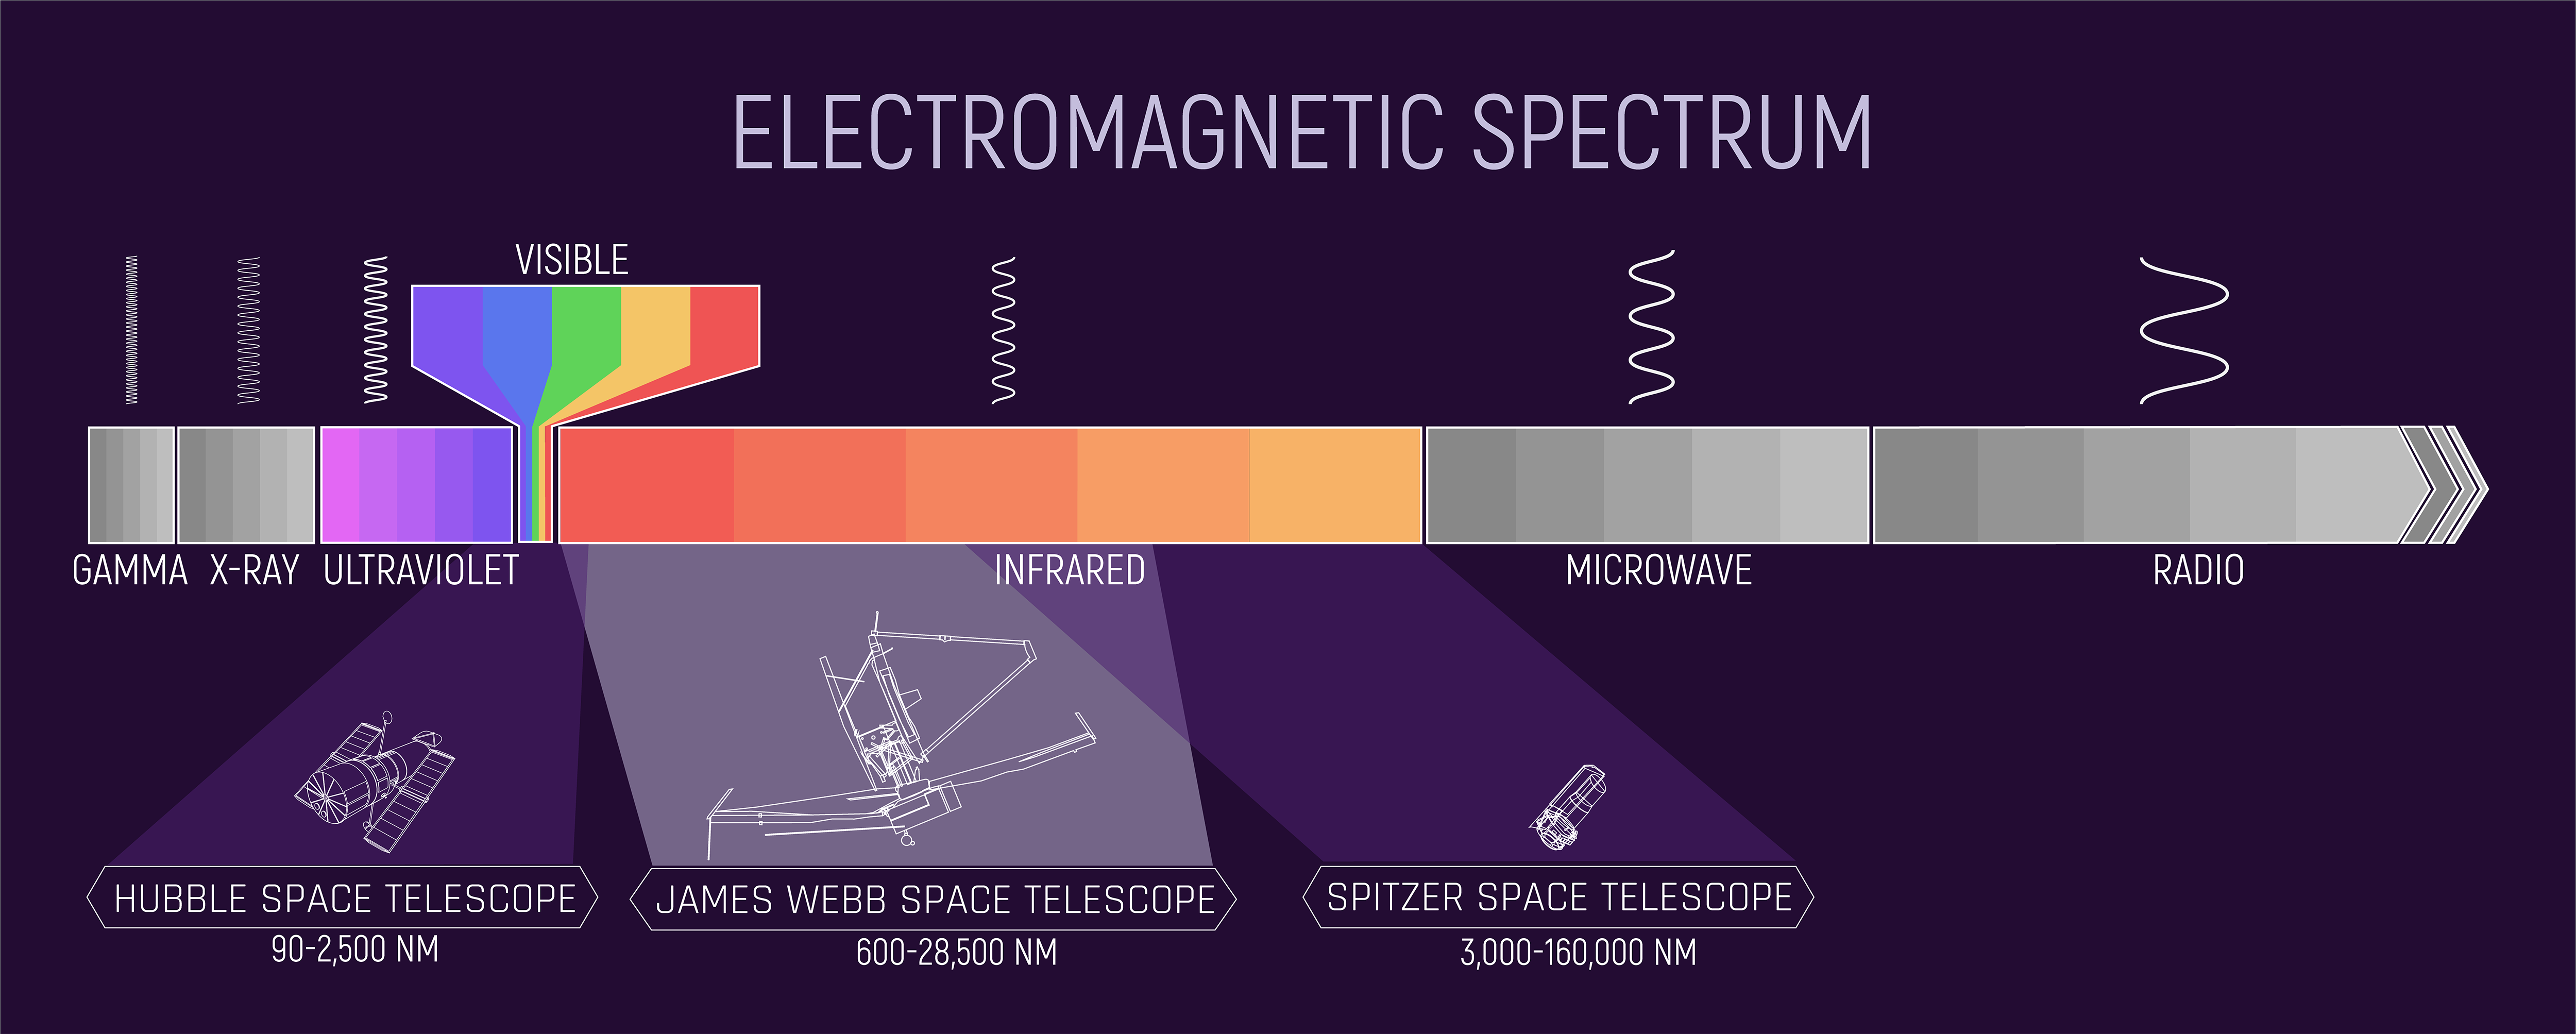
\includegraphics[width=1.0\textwidth]{wave_jwst.png}
                    \scriptsize \textit{Source: NASA/JPL-Caltech//R. Hurt (Caltech-IPAC)}
                    
                    \scriptsize \textit{Source: NASA, ESA, CSA, Joseph Olmsted (STScI)}
            \end{center}
        \end{column}
    
        % --- Left Column (Text) ---
        \begin{column}{0.5\textwidth}
            \textbf{What is redshift?}
            \begin{itemize}
                \item \textbf{Stretching} of light waves as an object moves away from the observer. 
                \item Light's wavelength gets stretched, so it \textbf{shifts} toward the red end of the light spectrum.
                \item Redder light = More distant galaxies. 
                \item Bluer light = Closer galaxies.
            \end{itemize}
        \end{column}
        

    \end{columns}
\end{frame}


% --- Slide 10: Little Red Dots ---
\begin{frame}
    \frametitle{Little Red Dots}
    
    \begin{columns}
    
        % --- Left Column (Images) ---
        \begin{column}{0.6\textwidth}
            \begin{center}
                % First Image
                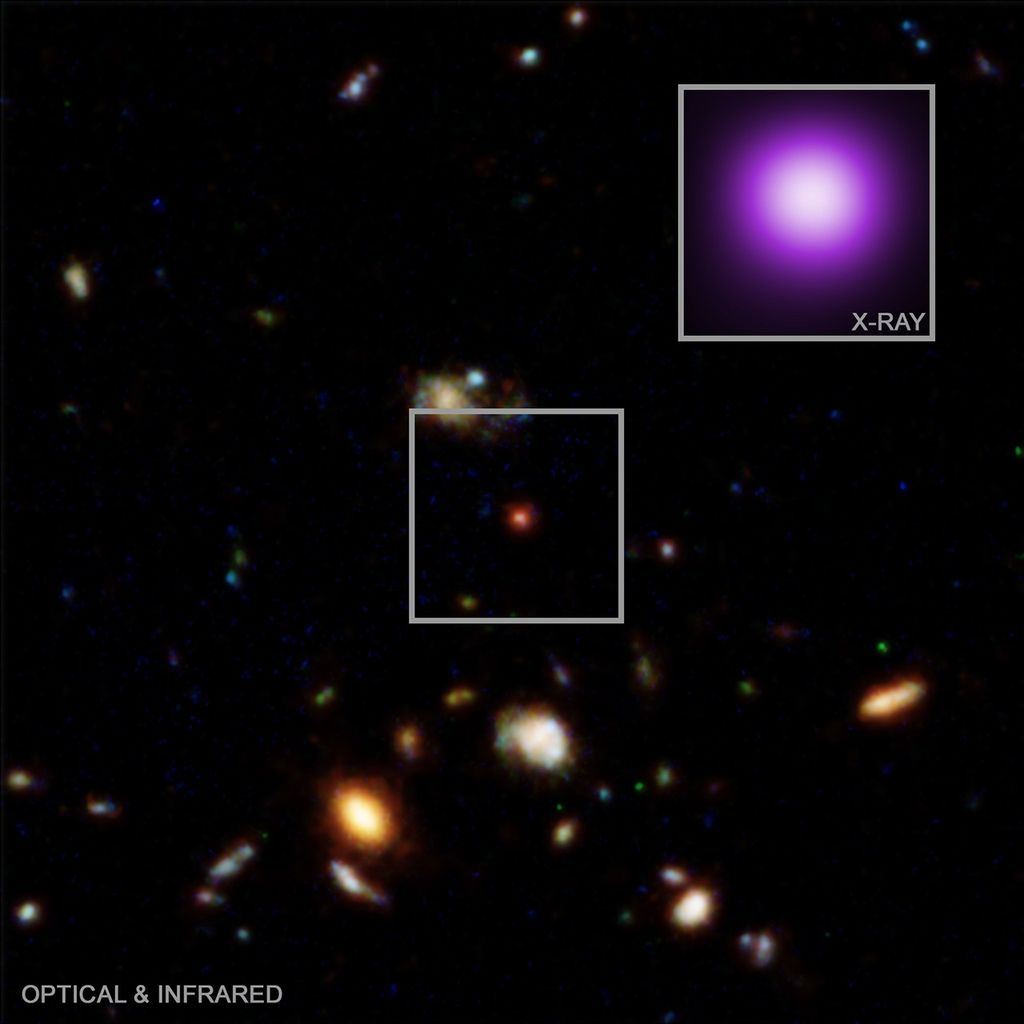
\includegraphics[width=0.4\textwidth]{infared_lrd.png} \\
                \vspace{0.2cm} % Adds a tiny bit of vertical space so it isn't squished
                \tiny{Source: X-ray: NASA/CXC/Max Plank Inst./R. Hviding et al.; Optical/IR; NASA/ESA/STScI/HST; Image Processing: NASA/CXC/SAO/N. Wolk} % Makes the text small and italicized
                \vspace{0.2cm} % Small cushion between images
                
                % Second Image
                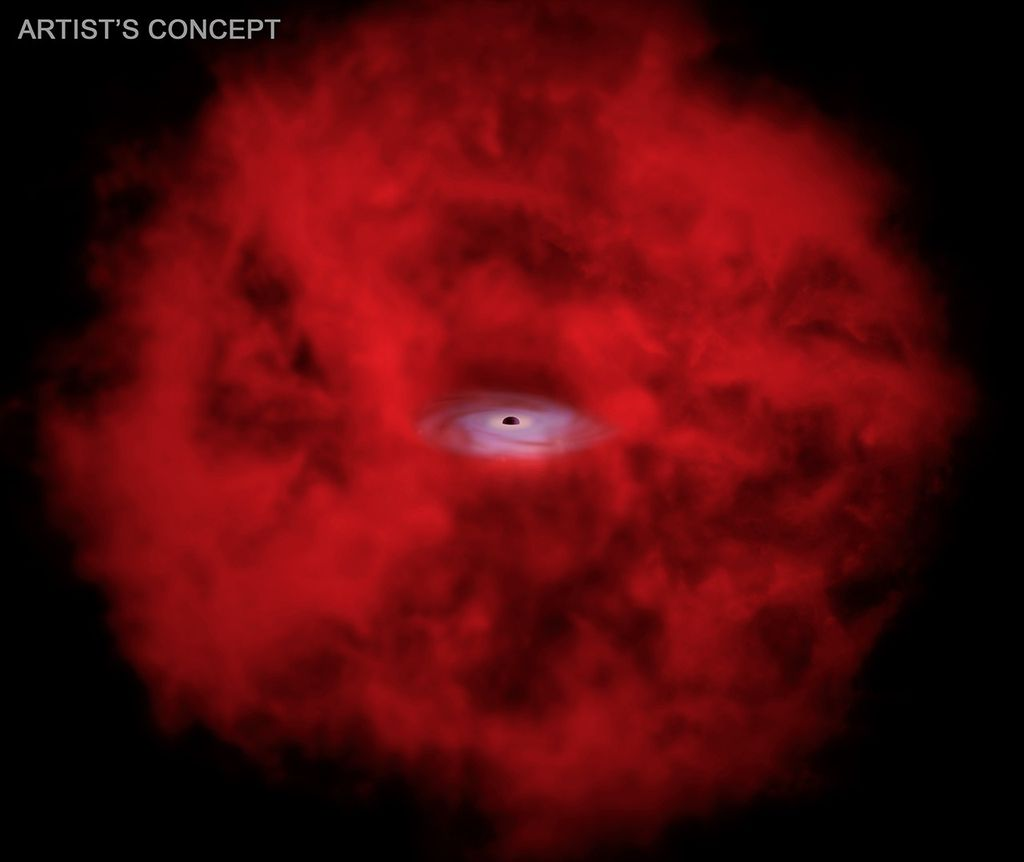
\includegraphics[width=0.5\textwidth]{lrd_art.png}
                \tiny{Source: NASA/CXC/SAO/M. Weiss; adapted by K. Arcand & J. Major}
            \end{center}
        \end{column}
        
        % --- Right Column (Text) ---
        \begin{column}{0.4\textwidth}
            \begin{item}
                \item Deep space objects recently discovered by the James Webb Space Telescope (JWST). 
            \end{item}
            \begin{itemize}
                \item Star Forming
                \item Composite Region
                \item BLAGN Region
            \end{itemize}
        \end{column}
    \end{columns}
\end{frame}


% --- Slide 12: Hydrogen Lines ---
\begin{frame}
    \frametitle{Hydrogen Lines}
    As electrons move through the orbitals, they produce light with a specific shade of color. 
    \begin{itemize}
        \item Hydrogen $\alpha$ 
        \item Hydrogen $\beta$ 
        \item \textbf{Hydrogen $\gamma$}
    \end{itemize}
    
    % The negative number pulls the image UP!
    \vspace{-3.3cm}
    
    % start image
    \begin{center} 
        \hspace*{2.4cm} 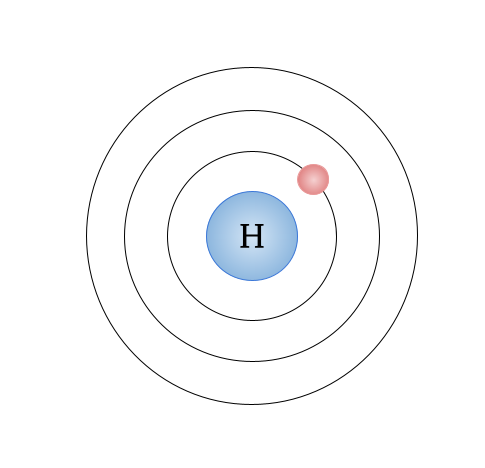
\includegraphics[width=0.8\textwidth]{hydro_shell.png}
    \end{center}
\end{frame}

% --- Slide 13: Oxygen III Lines ---
\begin{frame}
    \frametitle{[$OIII$] Lines}
    \begin{itemize}
        \item  In the [$OIII$] $\lambda$4363 emission, electrons are bumped up to high-energy excited states when they collide with fast-moving free electrons. 
        \item Collisional excitation
        \item The excited electron drops back down
    \end{itemize}

     \vspace{-0.6cm}
    % start image
    \begin{center} 
        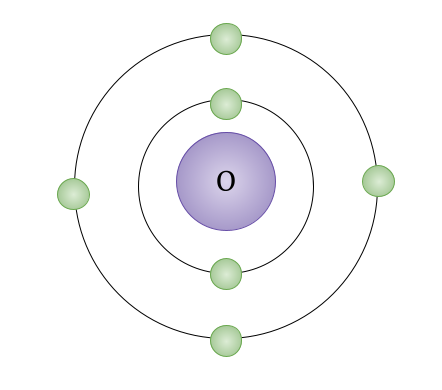
\includegraphics[width=0.65\textwidth]{oxy_shell.png}
    \end{center}
\end{frame}


% --- Slide 14: Plain Spectra ---
\begin{frame}
    \frametitle{Plain Spectra}
    % start image
    \begin{center} 
        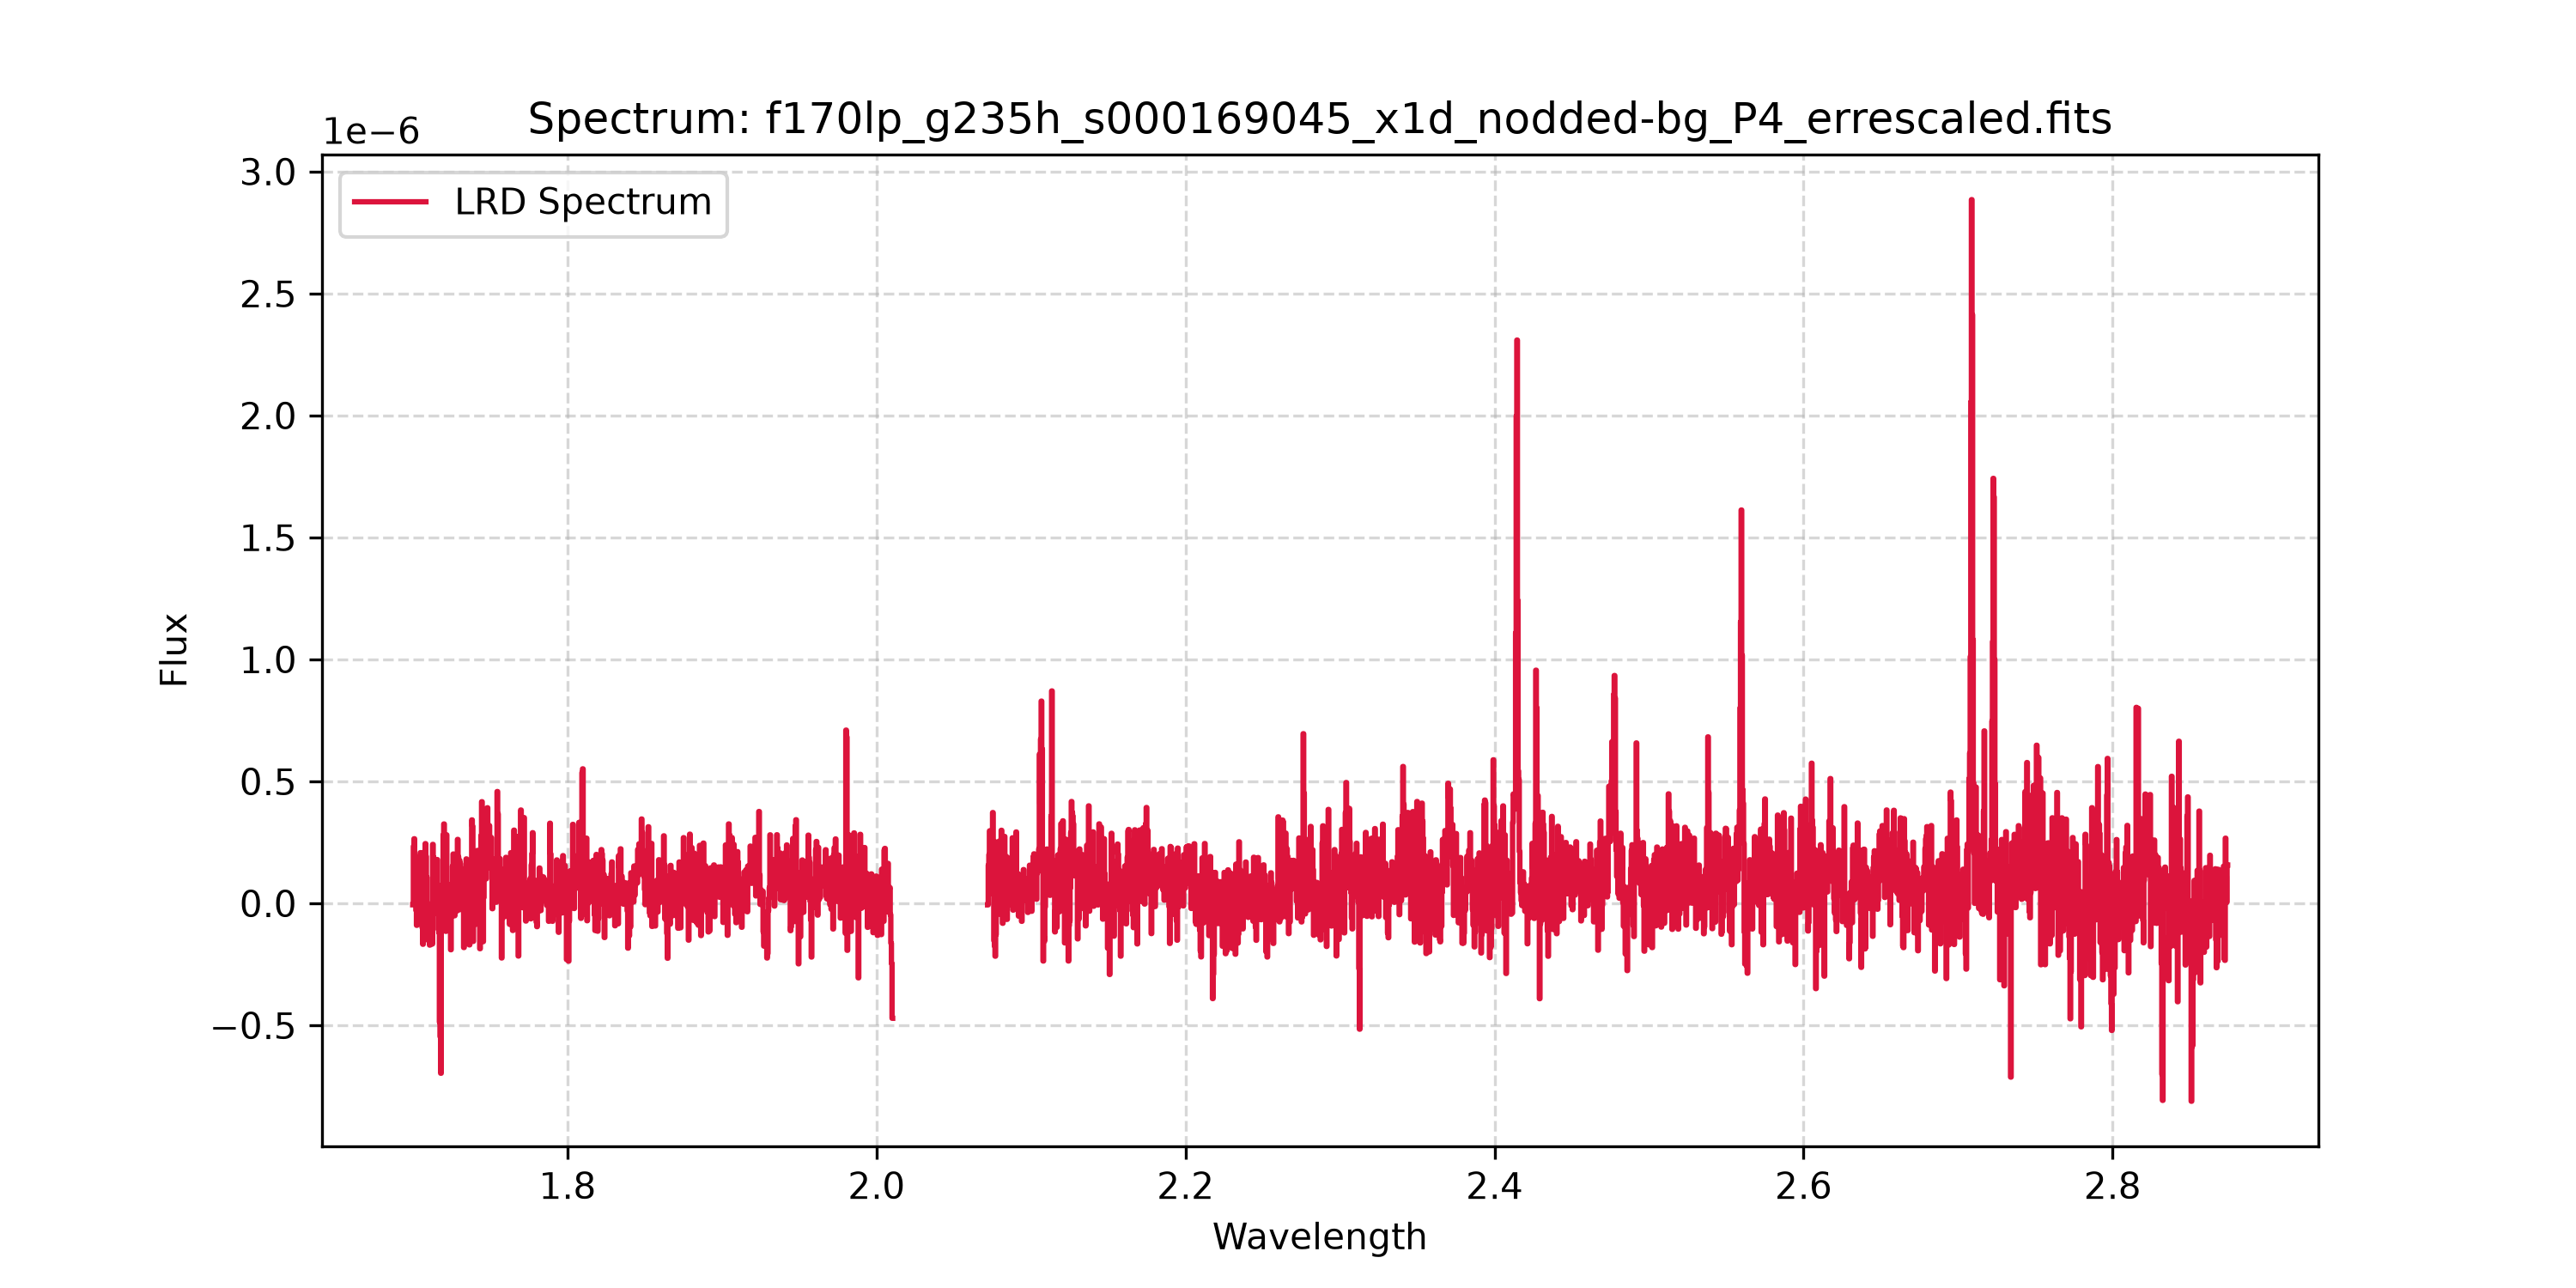
\includegraphics[width=1.0\textwidth]{plain_spectra.png}
    \end{center}

\end{frame}

% --- Slide 15: Gamma Spectra ---
\begin{frame}
    \frametitle{Spectra with Hydrogen $\gamma$ Identified}
    % start image
    \begin{center} 
        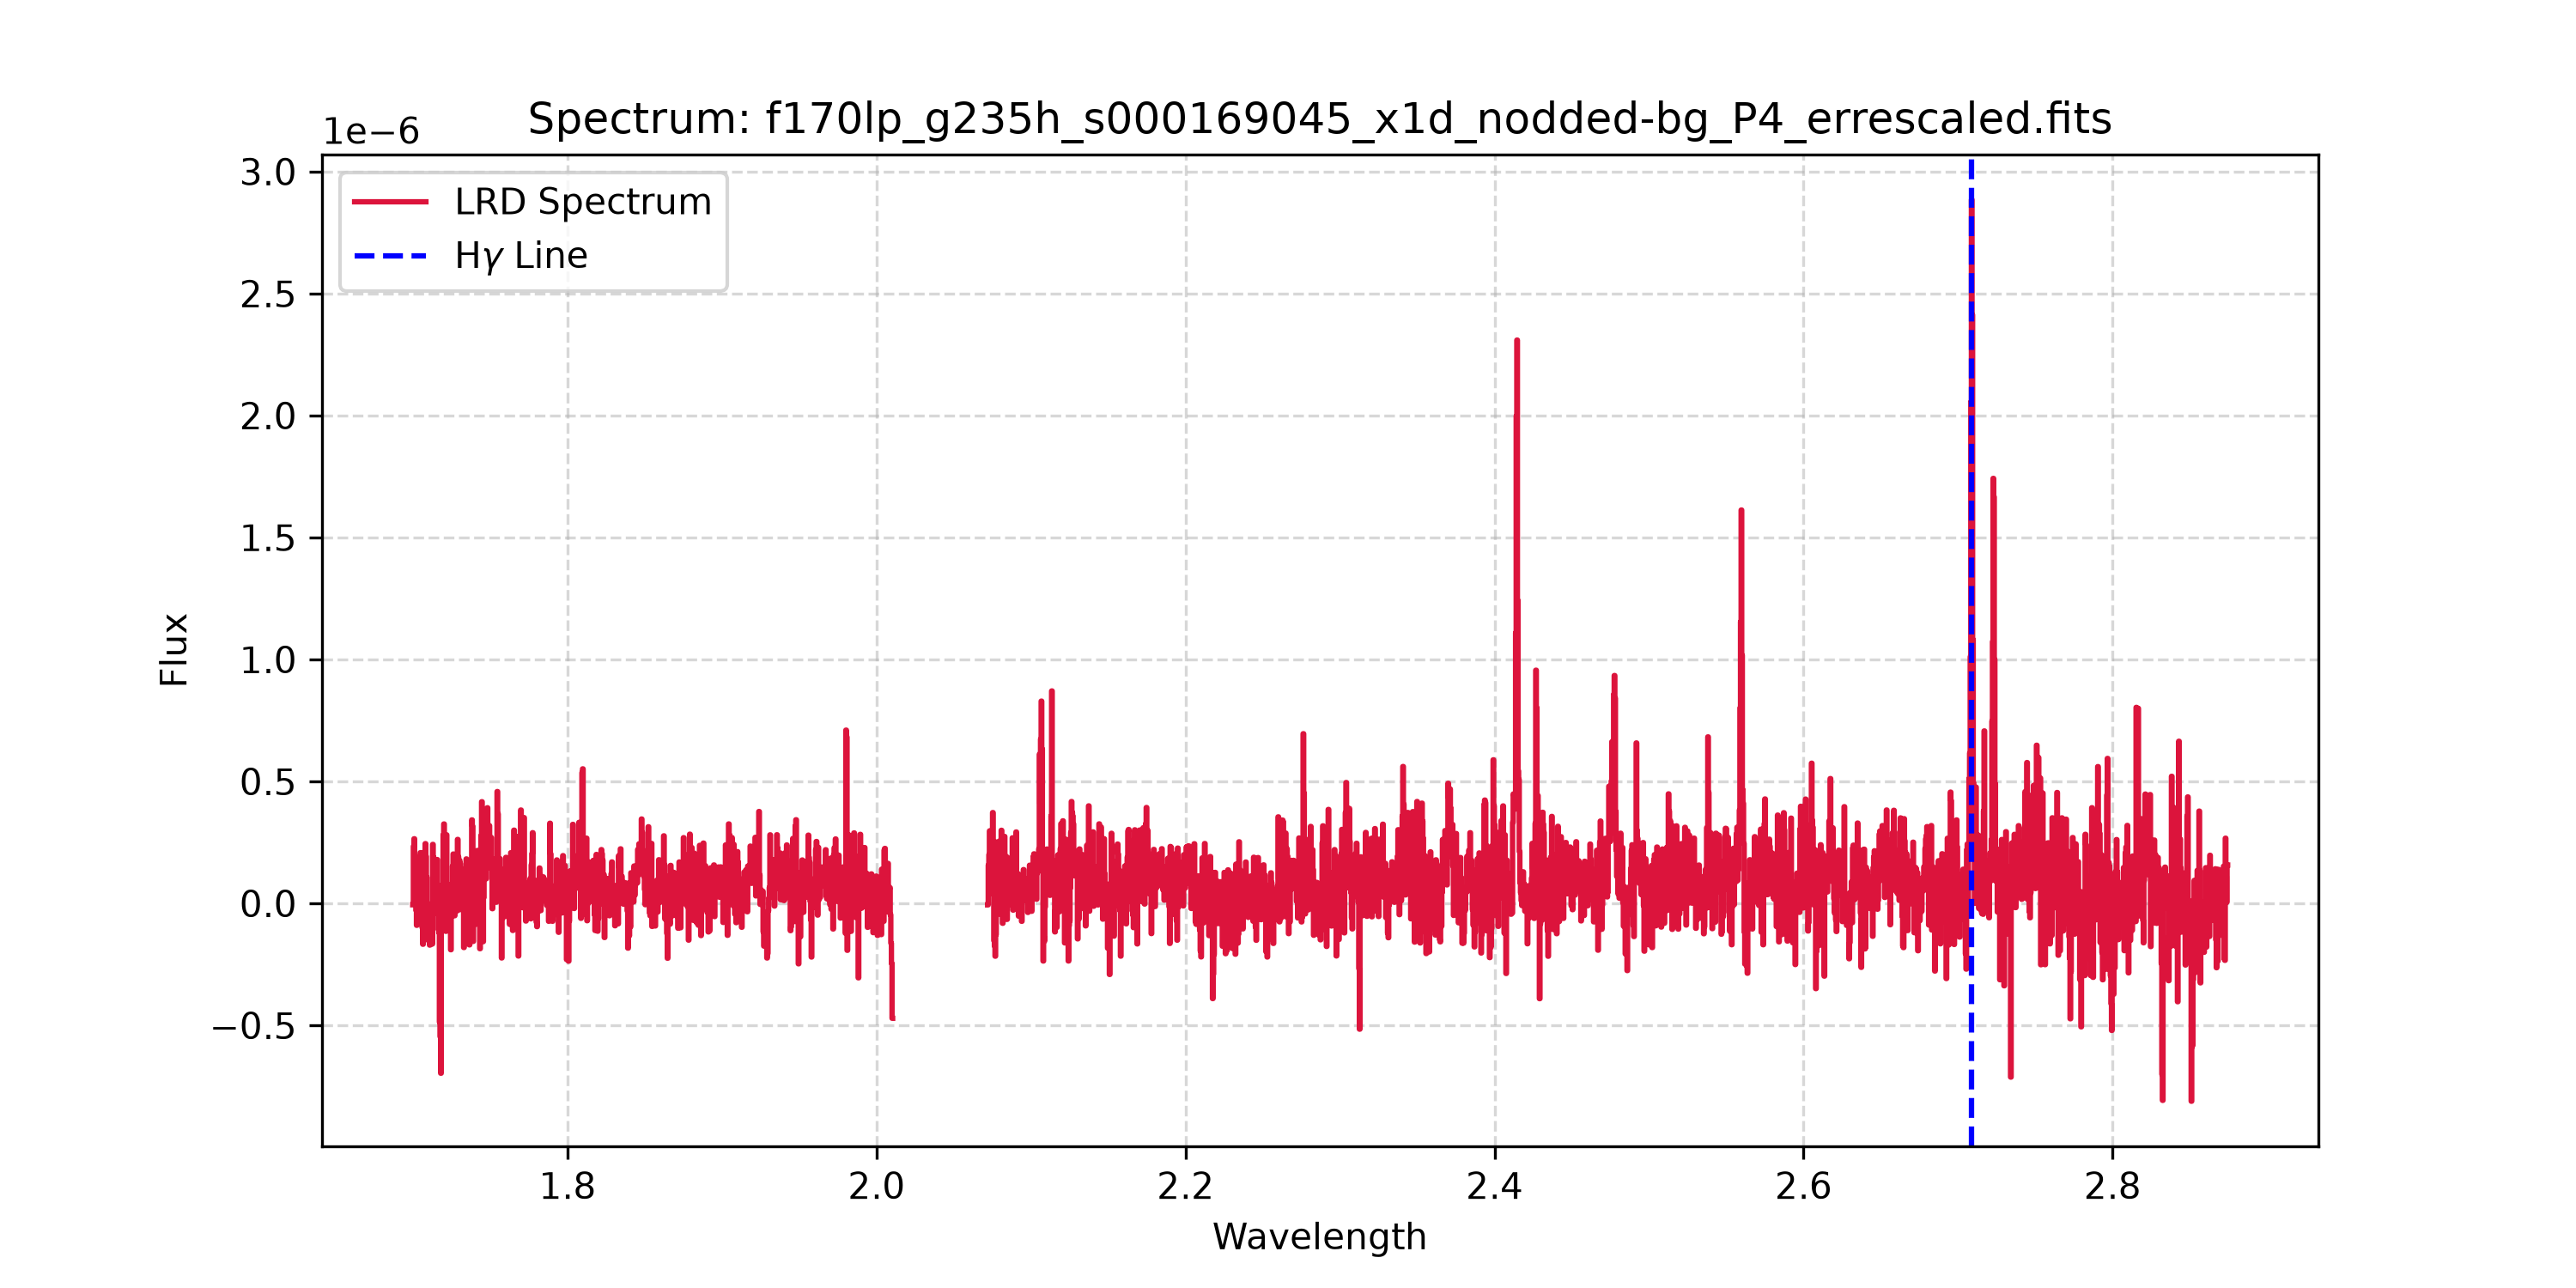
\includegraphics[width=1.0\textwidth]{gamma_spectra.png}
    \end{center}

\end{frame}

% --- Slide 16: O3 Spectra ---
\begin{frame}
    \frametitle{Spectra with [$OIII$] Identified}
    % start image
    \begin{center} 
        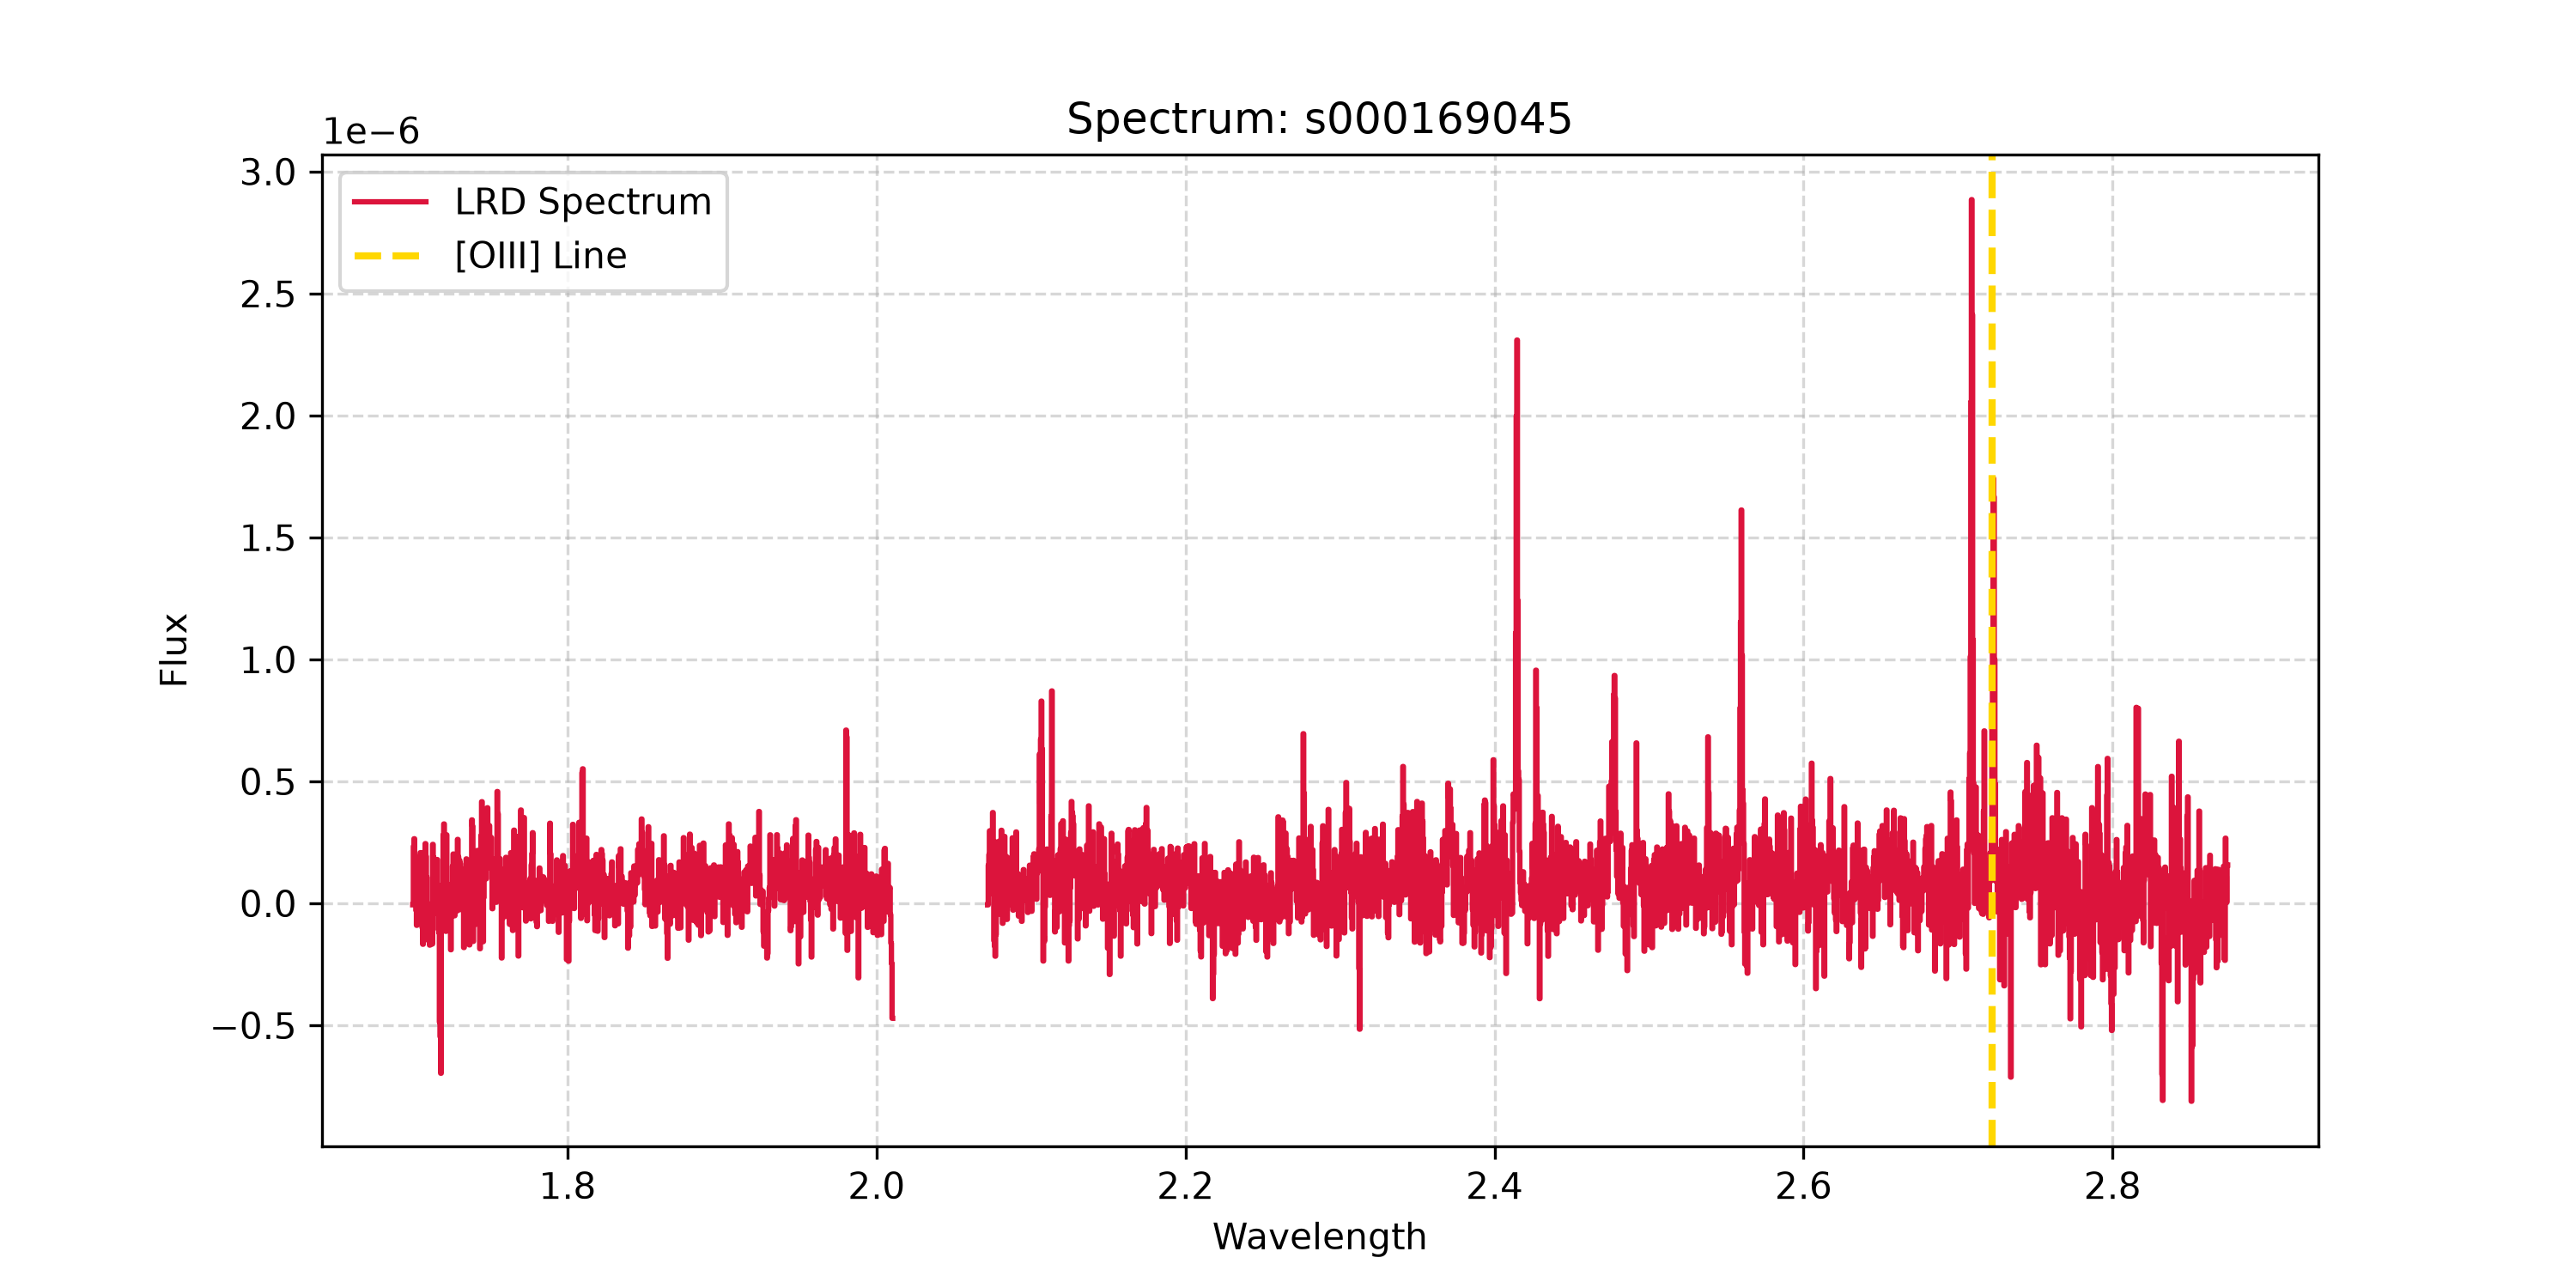
\includegraphics[width=1.0\textwidth]{oxy_spectra.png}
    \end{center}

\end{frame}

% --- Slide 17: Both Spectra ---
\begin{frame}
    \frametitle{Spectra with Both Emissions Identified}
    % start image
    \begin{center} 
        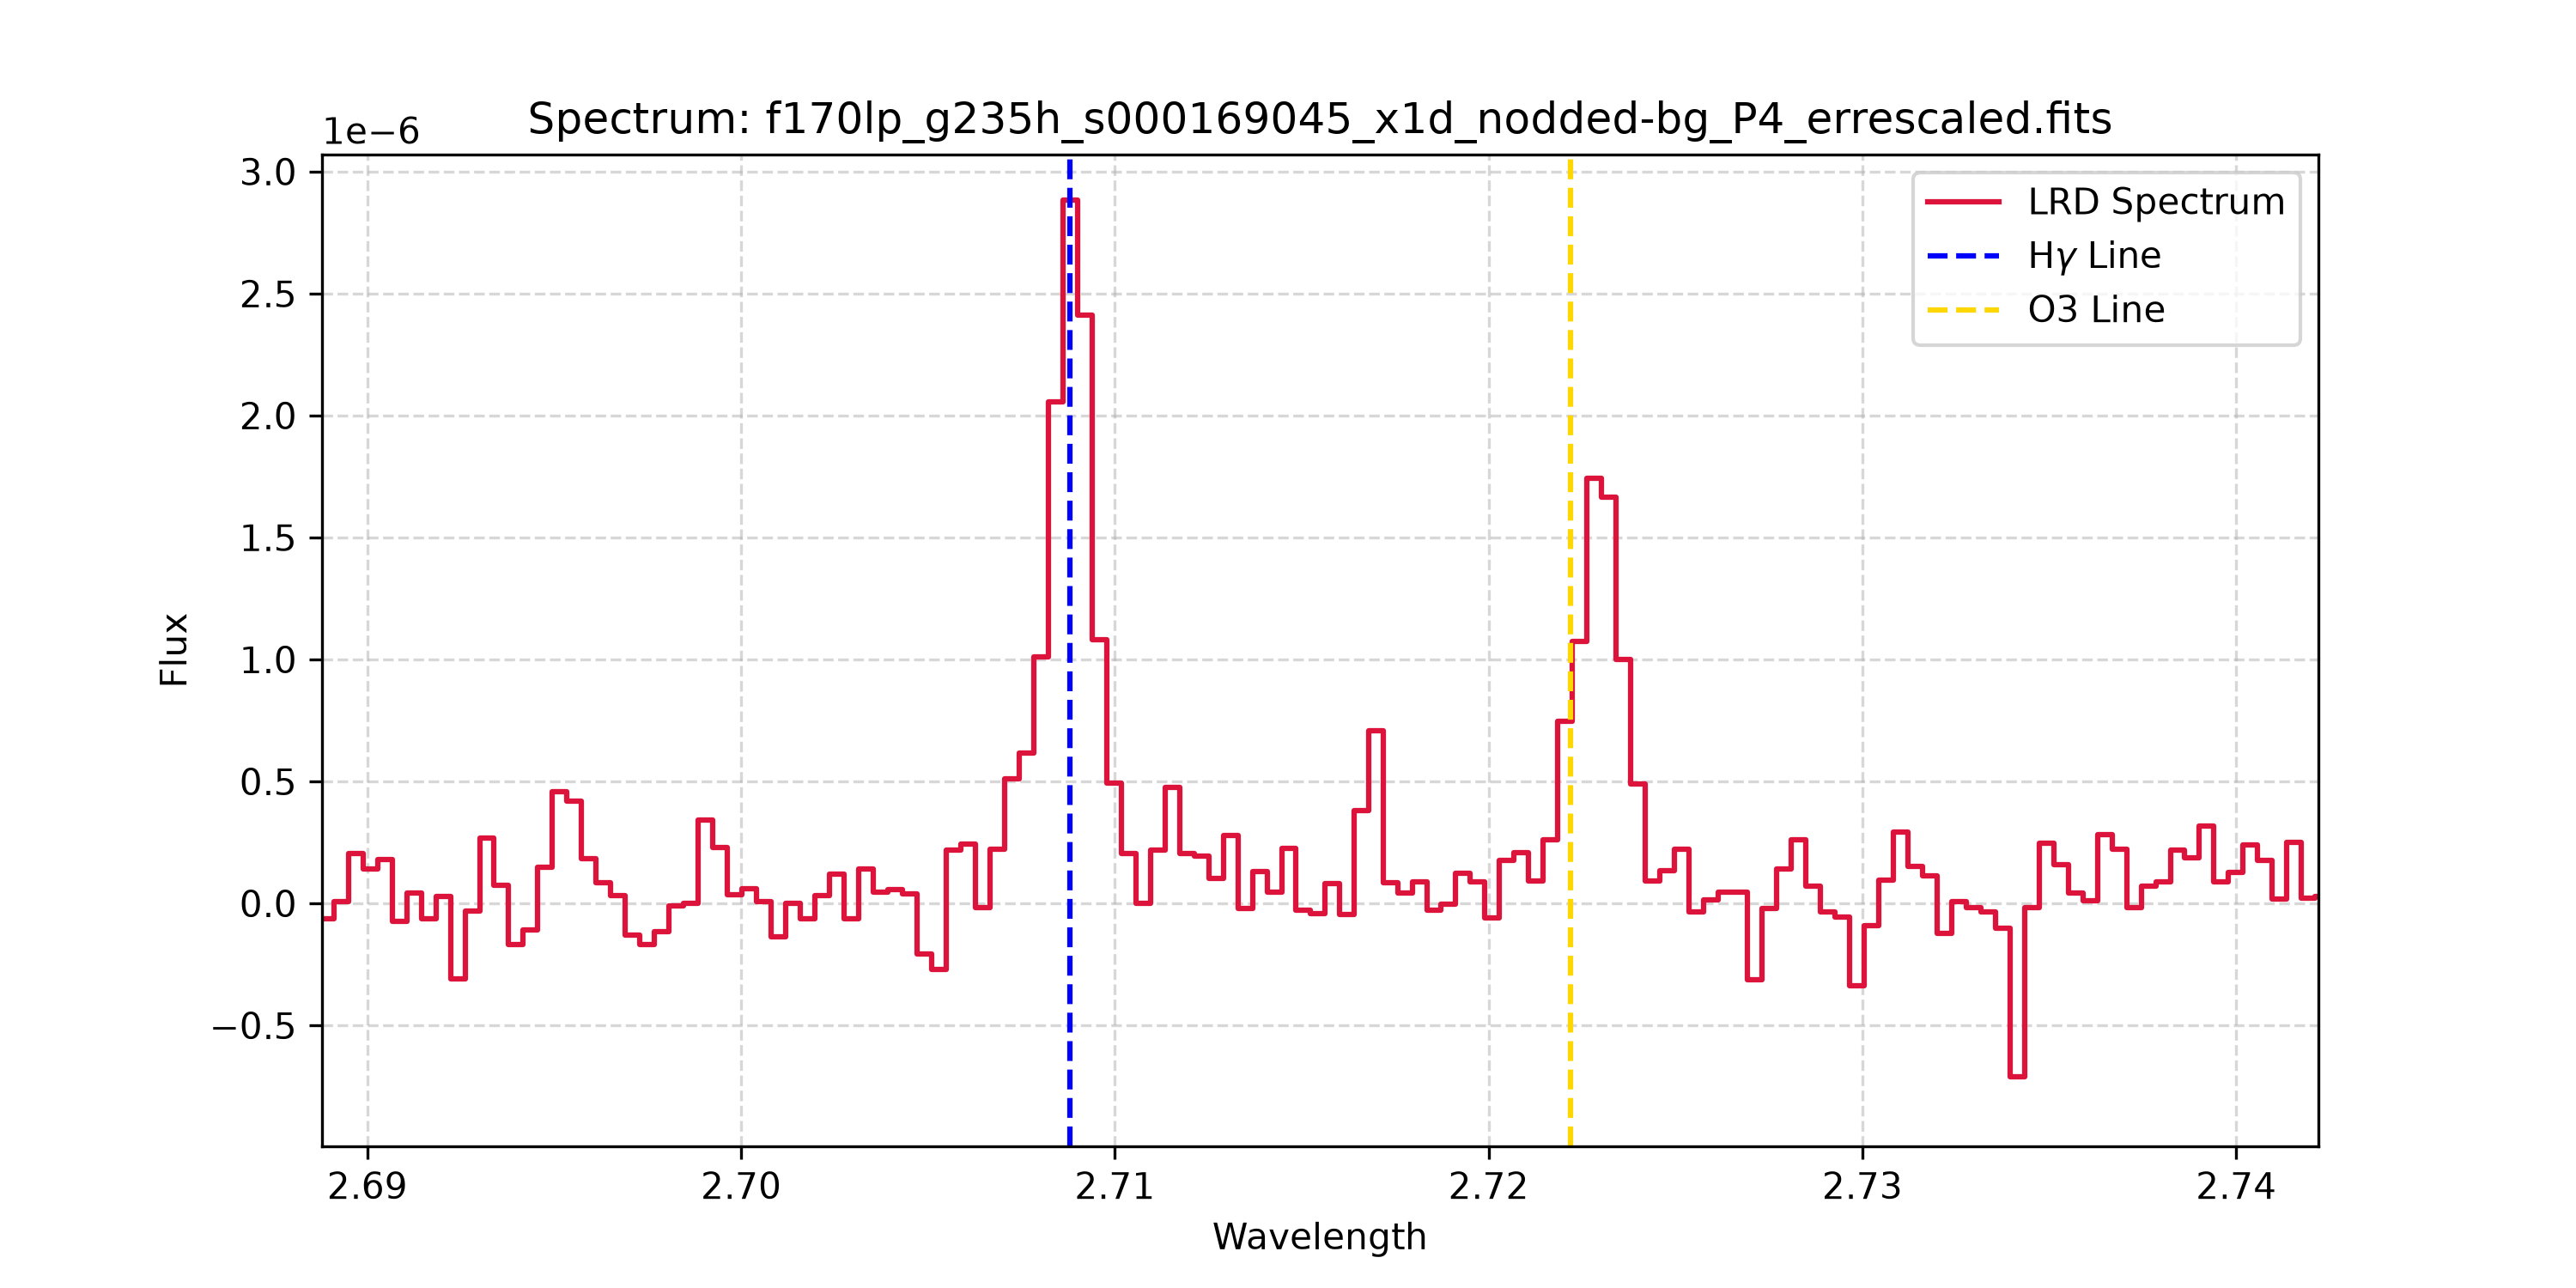
\includegraphics[width=1.0\textwidth]{both_spectra.png}
    \end{center}

\end{frame}

% --- Slide 5: Absorption ---
\begin{frame}
    \frametitle{Standout LRDs}
    % start image
    \begin{center} 
        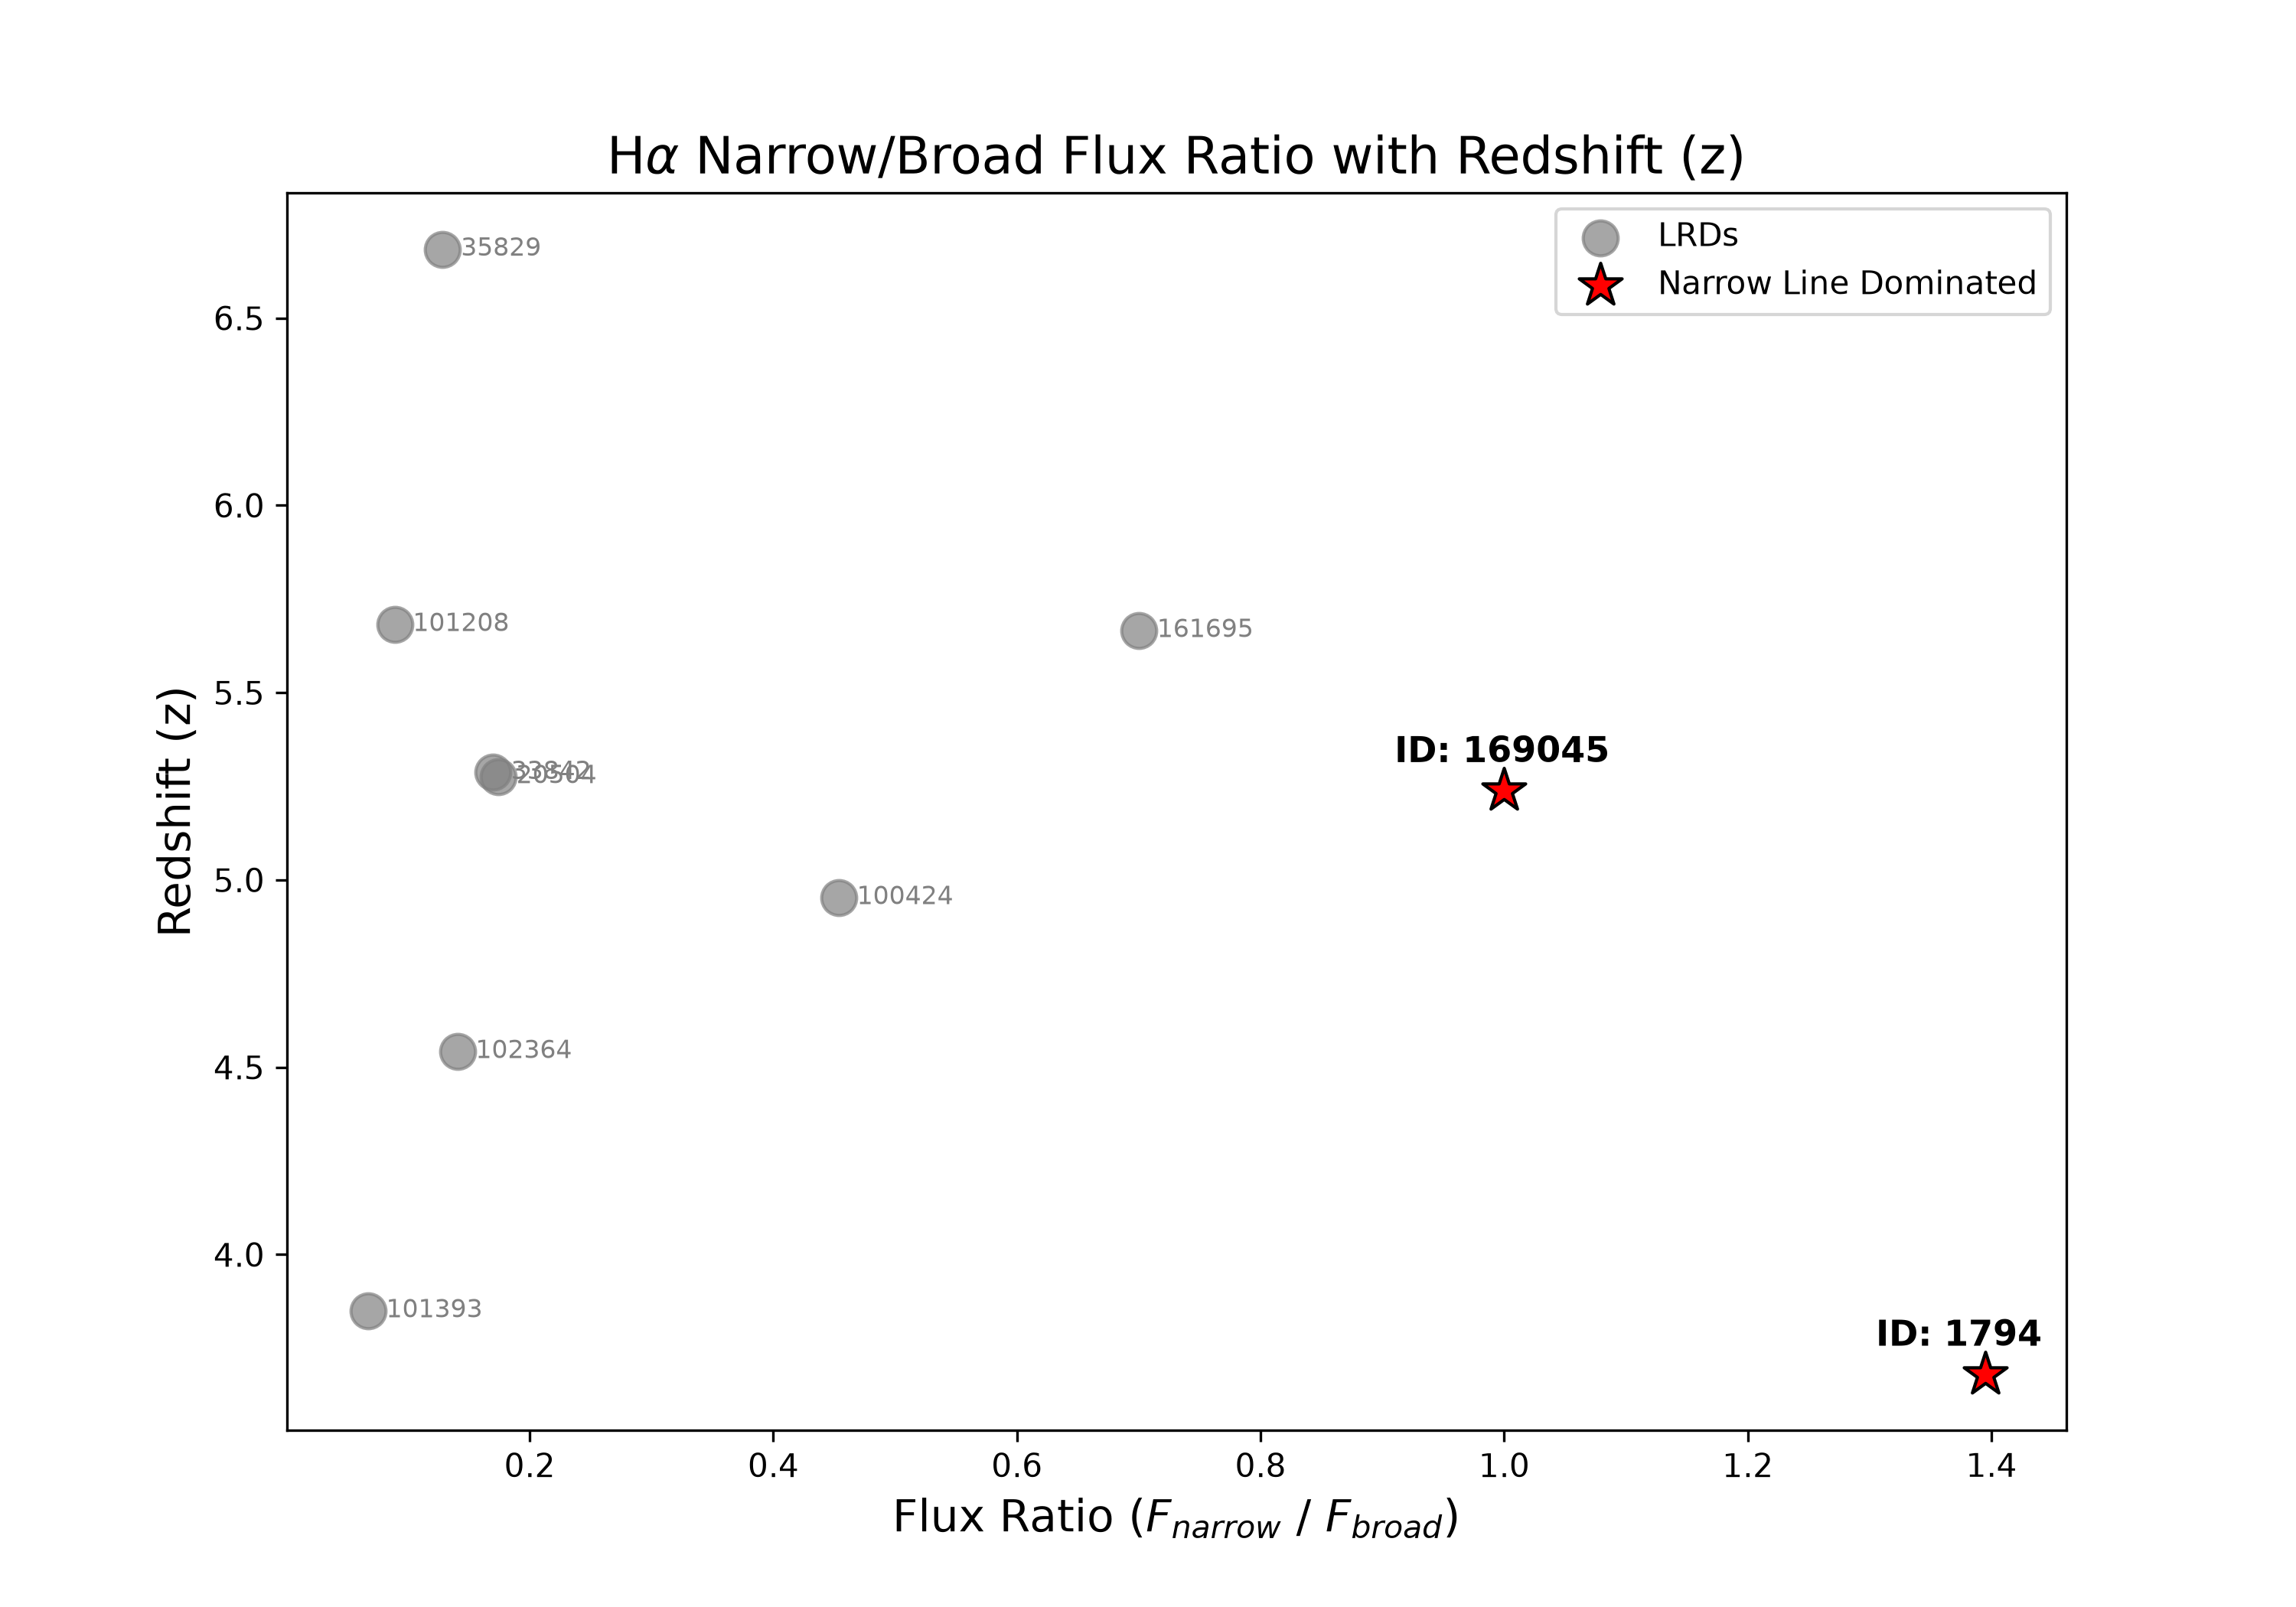
\includegraphics[width=0.7\textwidth]{Halpha_ratio.png}
        \vspace{0.2cm} % Adds a tiny bit of vertical space so it isn't squished
    \end{center}
    
    \begin{itemize}
        \item Two standout sources
    \end{itemize}
    
    \vspace{0.2cm} 
\end{frame}

% --- Slide 18: Line Plot ---
\begin{frame}
    \frametitle{Line Plot}
    % start image
    \begin{center} 
        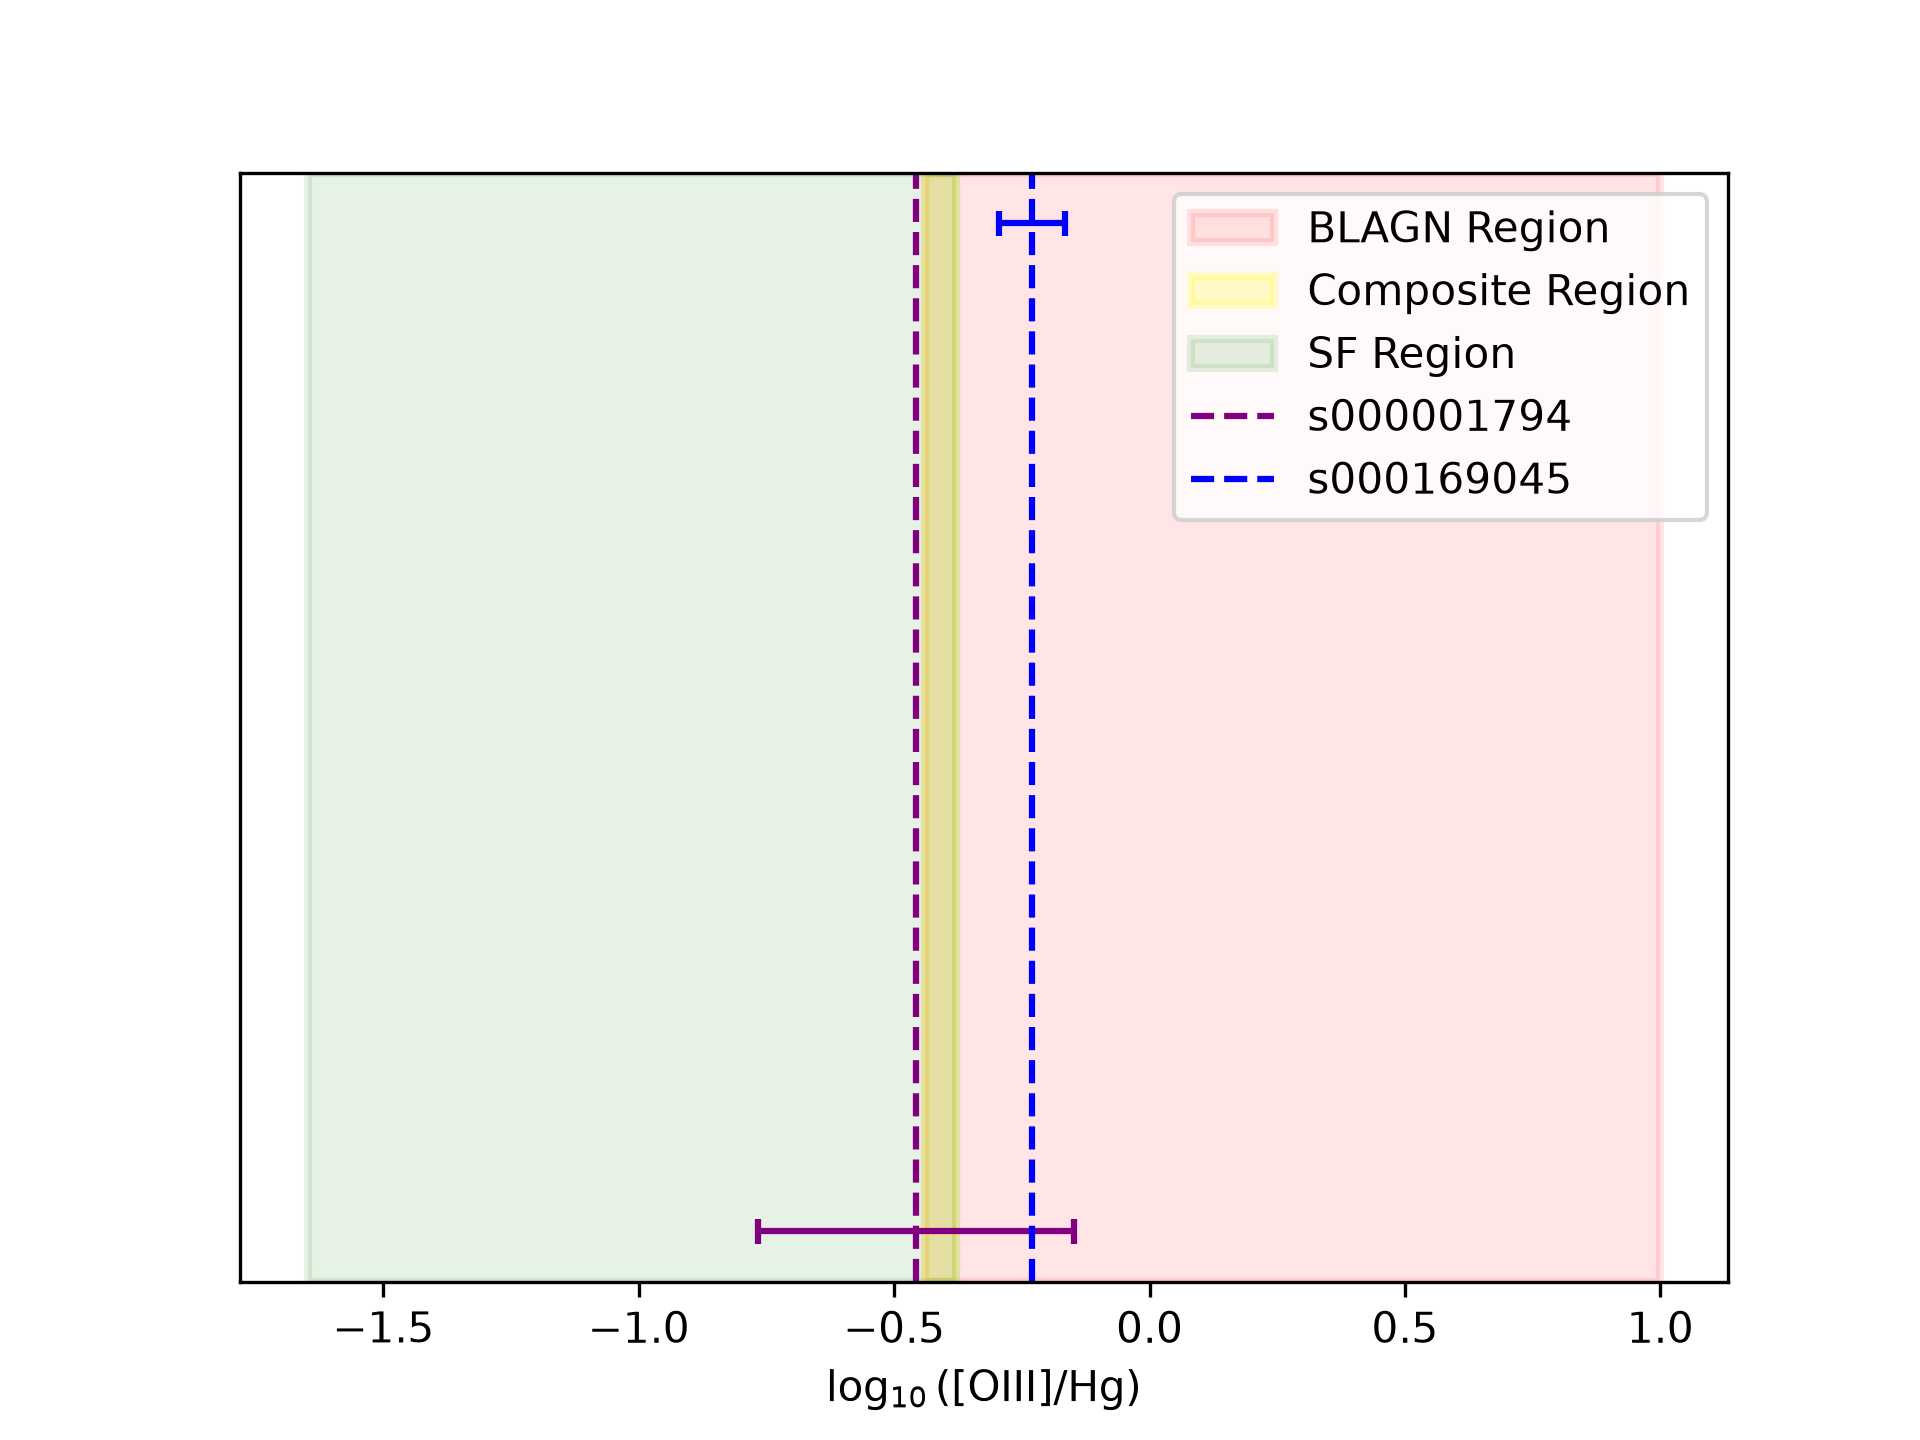
\includegraphics[width=.9\textwidth]{histo.png}
    \end{center}

\end{frame}

% --- Slide 20: References ---
\begin{frame}
    \frametitle{References}
    \begin{itemize}
    \item Backhaus, B. E., Cleri, N. J., Trump, J. R., et al. 2025,
Emission-Line Diagnostics at z¿4: [OIII]λ4363/Hγ, arXive −
prints. https://arxiv.org/abs/2502.03519https://arxiv.org/abs/2502.03519
    \item Davis, K., Brooks, M., Simons, R. C., et al. 2026, OCEANS of Absorption: High-resolution NIRSpec
    \item Hunter, J. D. 2007, Matplotlib: A 2D graphics environment, Computing in Science & Engineering, 9, 90, doi: http://doi.org/10.1109/MCSE.2007.5510.1109/MCSE.2007.55
Spectroscopy Reveals Diverse Balmer-line Absorption in Little Red Dots, arXiv e-prints, arXiv:2606.00258, doi: http://doi.org/10.48550/arXiv.2606.0025810.48550/arXiv.2606.00258
    \item Fern´andez, V., Amor´ın, R., Firpo, V., & Morisset, C. 2024, LIME: A LIne MEasuring library for large and complex spectroscopic data sets. I. Implementation of a virtual observatory for JWST spectra, , 688, A69, doi: http://doi.org/10.1051/0004-6361/20244922410.1051/0004-6361/202449224
    \end{itemize}
\end{frame}

% --- Slide 19: Questions? ---
\begin{frame}
    \begin{center}
        \Huge{Questions?}
    \end{center}
\end{frame}

\end{document}